\documentclass[leqno, openany]{memoir}
\setulmarginsandblock{3.5cm}{3.5cm}{*}
\setlrmarginsandblock{3cm}{3.5cm}{*}
\checkandfixthelayout

\usepackage{amsmath}
\usepackage{amssymb}
\usepackage{amsthm}
%\usepackage{MnSymbol}
\usepackage{bm}
\usepackage{accents}
\usepackage{mathtools}
\usepackage{tikz}
\usetikzlibrary{decorations.pathmorphing,shapes}
\usetikzlibrary{calc}
\usetikzlibrary{automata,positioning}
\usepackage{tikz-cd}
\usepackage{forest}
\usepackage{braket} 
\usepackage{listings}
\usepackage{mdframed}
\usepackage{verbatim}
\usepackage{physics}
\usepackage{stmaryrd}
\usepackage{mathrsfs} 
\usepackage{stackengine} 
%\usepackage{/home/patrickl/homework/macaulay2}

%font
\usepackage[sc]{mathpazo}
\usepackage{eulervm}
\usepackage[scaled=0.86]{berasans}
\usepackage{inconsolata}
\usepackage{microtype}

%CS packages
\usepackage{algorithmicx}
\usepackage{algpseudocode}
\usepackage{algorithm}

% typeset and bib
\usepackage[english]{babel} 
\usepackage[utf8]{inputenc} 
\usepackage[T1]{fontenc}
\usepackage[backend=biber, style=alphabetic]{biblatex}
\usepackage[bookmarks, colorlinks, breaklinks]{hyperref} 
\hypersetup{linkcolor=black,citecolor=black,filecolor=black,urlcolor=black}

% other formatting packages
\usepackage{float}
\usepackage{booktabs}
\usepackage[shortlabels]{enumitem}
\usepackage{csquotes}
\usepackage{titlesec}
\usepackage{titling}
\usepackage{fancyhdr}
\usepackage{lastpage}
\usepackage{parskip}
\usepackage{graphicx}
\graphicspath{{./images/}}

\usepackage{lipsum}

% delimiters
\DeclarePairedDelimiter{\gen}{\langle}{\rangle}
\DeclarePairedDelimiter{\floor}{\lfloor}{\rfloor}
\DeclarePairedDelimiter{\ceil}{\lceil}{\rceil}


\newtheorem{thm}{Theorem}[section]
\newtheorem{cor}[thm]{Corollary}
\newtheorem{prop}[thm]{Proposition}
\newtheorem{lem}[thm]{Lemma}
\newtheorem{conj}[thm]{Conjecture}
\newtheorem{quest}[thm]{Question}

\theoremstyle{definition}
\newtheorem{defn}[thm]{Definition}
\newtheorem{defns}[thm]{Definitions}
\newtheorem{con}[thm]{Construction}
\newtheorem{exm}[thm]{Example}
\newtheorem{exms}[thm]{Examples}
\newtheorem{notn}[thm]{Notation}
\newtheorem{notns}[thm]{Notations}
\newtheorem{addm}[thm]{Addendum}
\newtheorem{exer}[thm]{Exercise}

\theoremstyle{remark}
\newtheorem{rmk}[thm]{Remark}
\newtheorem{rmks}[thm]{Remarks}
\newtheorem{warn}[thm]{Warning}
\newtheorem{sch}[thm]{Scholium}


% unnumbered theorems
\theoremstyle{plain}
\newtheorem*{thm*}{Theorem}
\newtheorem*{prop*}{Proposition}
\newtheorem*{lem*}{Lemma}
\newtheorem*{cor*}{Corollary}
\newtheorem*{conj*}{Conjecture}

% unnumbered definitions
\theoremstyle{definition}
\newtheorem*{defn*}{Definition}
\newtheorem*{exer*}{Exercise}
\newtheorem*{defns*}{Definitions}
\newtheorem*{con*}{Construction}
\newtheorem*{exm*}{Example}
\newtheorem*{exms*}{Examples}
\newtheorem*{notn*}{Notation}
\newtheorem*{notns*}{Notations}
\newtheorem*{addm*}{Addendum}


\theoremstyle{remark}
\newtheorem*{rmk*}{Remark}

% shortcuts
\newcommand{\Ima}{\mathrm{Im}}
\newcommand{\A}{\mathbb{A}}
\newcommand{\G}{\mathbb{G}}
\newcommand{\N}{\mathbb{N}}
\newcommand{\R}{\mathbb{R}}
\newcommand{\C}{\mathbb{C}}
\newcommand{\Z}{\mathbb{Z}}
\newcommand{\Q}{\mathbb{Q}}
\renewcommand{\k}{\Bbbk}
\renewcommand{\P}{\mathbb{P}}
\newcommand{\M}{\overline{M}}
\newcommand{\g}{\mathfrak{g}}
\newcommand{\h}{\mathfrak{h}}
\newcommand{\n}{\mathfrak{n}}
\renewcommand{\b}{\mathfrak{b}}
\newcommand{\ep}{\varepsilon}
\newcommand*{\dt}[1]{%
   \accentset{\mbox{\Huge\bfseries .}}{#1}}
\renewcommand{\abstractname}{Official Description}
\newcommand{\mc}[1]{\mathcal{#1}}
\newcommand{\T}{\mathbb{T}}
\newcommand{\mf}[1]{\mathfrak{#1}}
\newcommand{\mr}[1]{\mathrm{#1}}
\newcommand{\ms}[1]{\mathsf{#1}}
\newcommand{\ol}[1]{\overline{#1}}
\newcommand{\ul}[1]{\underline{#1}}
\newcommand{\wt}[1]{\widetilde{#1}}
\newcommand{\wh}[1]{\widehat{#1}}
\renewcommand{\div}{\operatorname{div}}
\newcommand{\Sm}{\mathsf{Sm}}
\newcommand{\Cor}{\mathsf{Cor}}

\DeclareMathOperator{\Der}{Der}
\DeclareMathOperator{\Hom}{Hom}
\DeclareMathOperator{\End}{End}
\DeclareMathOperator{\ad}{ad}
\DeclareMathOperator{\Aut}{Aut}
\DeclareMathOperator{\Rad}{Rad}
\DeclareMathOperator{\Pic}{Pic}
\DeclareMathOperator{\supp}{supp}
\DeclareMathOperator{\Supp}{Supp}
\DeclareMathOperator{\sgn}{sgn}
\DeclareMathOperator{\spec}{Spec}
\DeclareMathOperator{\rk}{rk}
\DeclareMathOperator{\Spec}{Spec}
\DeclareMathOperator{\proj}{Proj}
\DeclareMathOperator{\Proj}{Proj}
\DeclareMathOperator{\ord}{ord}
\DeclareMathOperator{\Div}{Div}
\DeclareMathOperator{\Bl}{Bl}
\DeclareMathOperator{\ch}{ch}
\DeclareMathOperator{\td}{td}
\DeclareMathOperator{\Tor}{Tor}
\DeclareMathOperator{\depth}{depth}
\DeclareMathOperator{\CH}{CH}
\DeclareMathOperator{\Ob}{Ob}
\DeclareMathOperator{\Rat}{Rat} 
\DeclareMathOperator{\coker}{coker}
\DeclareMathOperator{\Hilb}{Hilb}
\DeclareMathOperator{\Sym}{Sym}

% Section formatting
\titleformat{\section}
    {\Large\sffamily\scshape\bfseries}{\thesection}{1em}{}
\titleformat{\subsection}[runin]
    {\large\sffamily\bfseries}{\thesubsection}{1em}{}
\titleformat{\subsubsection}[runin]{\normalfont\itshape}{\thesubsubsection}{1em}{}

\title{COURSE TITLE}
\author{Lectures by INSTRUCTOR, Notes by NOTETAKER}
\date{SEMESTER}

\newcommand*{\titleSW}
    {\begingroup% Story of Writing
    \raggedleft
    \vspace*{\baselineskip}
    {\Huge\itshape DAHA and Knot Homology Learning Seminar \\ Fall 2021}\\[\baselineskip]
    {\large\itshape Notes by Patrick Lei}\\[0.2\textheight]
    {\Large Lectures by Various}\par
    \vfill
    {\Large \sffamily Columbia University}
    \vspace*{\baselineskip}
\endgroup}
\pagestyle{simple}

\chapterstyle{ell}


%\renewcommand{\cftchapterpagefont}{}
\renewcommand\cftchapterfont{\sffamily}
\renewcommand\cftsectionfont{\scshape}
\renewcommand*{\cftchapterleader}{}
\renewcommand*{\cftsectionleader}{}
\renewcommand*{\cftsubsectionleader}{}
\renewcommand*{\cftchapterformatpnum}[1]{~\textbullet~#1}
\renewcommand*{\cftsectionformatpnum}[1]{~\textbullet~#1}
\renewcommand*{\cftsubsectionformatpnum}[1]{~\textbullet~#1}
\renewcommand{\cftchapterafterpnum}{\cftparfillskip}
\renewcommand{\cftsectionafterpnum}{\cftparfillskip}
\renewcommand{\cftsubsectionafterpnum}{\cftparfillskip}
\setrmarg{3.55em plus 1fil}
\setsecnumdepth{subsection}
\maxsecnumdepth{subsection}
\settocdepth{subsection}

\begin{document}
    
\begin{titlingpage}
\titleSW
\end{titlingpage}

\thispagestyle{empty}
\section*{Disclaimer}%
\label{sec:disclaimer}

These notes were taken during the seminar using the \texttt{vimtex} package of
the editor \texttt{neovim}.  Any errors are mine and not the speakers'.  In
addition, my notes are picture-free (but will include commutative diagrams) and
are a mix of my mathematical style and that of the lecturers.  If you find any
errors, please contact me at \texttt{plei@math.columbia.edu}.

I patched the notes from \'Alvaro's lecture using his notes, which contain some
material not covered during the lecture. The notes here only contain material
covered during the lecture.

\vspace*{1cm}

\noindent\textbf{Seminar Website:}\\
\url{https://math.columbia.edu/~samdehority/seminars/2021-fall-seminar-knot-homology} \newpage

\tableofcontents

\chapter{Sebastian (Sep 14): Khovanov Homology}%
\label{cha:sebastian_sep_14_khovanov_homology}

Recall that the \textit{Kauffman bracket} of a link diagram $D$ has axioms $\ev{\emptyset} = 1$, $\ev{0 \sqcup D} = (q+q^{-1}) \ev{D}$, and for any crossing
\[ \ev{\text{crossing}} = q \ev{\text{horizontal}} + q^{-1} \ev{\text{vertical}} \]
If $D$ has $n_+$ positive crossings and $n_-$ negative crossings, then the \textit{Jones polynomial} of the underlying link $L$ is $J(L) = {(-1)}^n q^{n_+ - 2n_-} \ev{D}$.

We may have heard that Khovanov homology is a categorification of the Jones polynomial. To motivate this, there are quantum invariants like the Jones polynomial, the HOMFLY polynomial, WRT, and others. On the other side, there are gauge-theoretic invariants like instanton Floer homology and the Casson invariant. The quantum invariants generally come from representations of quantum groups are are combinatorial, but it is unclear what geometric information we obtain. On the other hand, the gauge theoretic invariants are more powerful, but of course harder to compute. We want to consider relations between the two types of invariants.

Some of the gauge-theoretic invariants end up being Euler characteristics; for example, the Casson invariant is twice the Euler characteristic of instanton Floer homology.

For a link diagram $L$, we will introduce a bigraded $\Z$-module $\mr{ Kh }^{*,*}(L)$ such that 
\[ J(L) = \sum_{i,j} {(-1)}^i q^j \rk_{\Z} \mr{ Kh }^{i,j}(L). \]

\section{Category of Pictures}%
\label{sec:category_of_pictures}

Given $D$, we will order its crossings. For each crossing we have a $0$-resolution (horizontal) and a $1$-resolution (vertical). If $n = n_+ + n_-$, then each element of $\qty{0,1}^n$ gets a complete resolution, which is a collection of circles in the plane. For example, consider the Hopf link with resolution. 

% insert picture here
\begin{figure}[H]
    \centering
    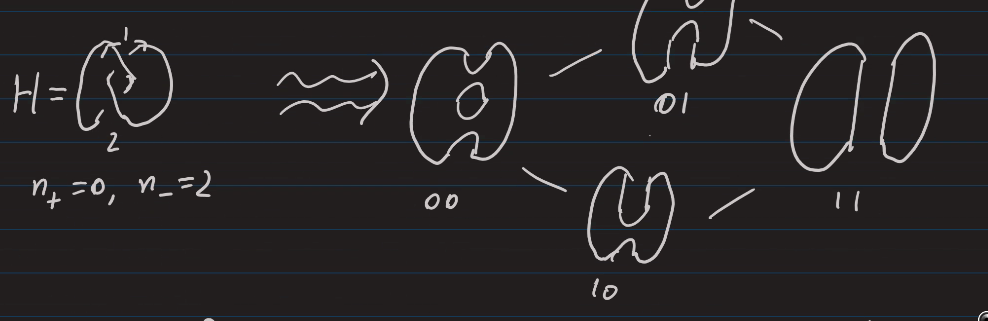
\includegraphics[width=0.8\linewidth]{seb1.png}
    \caption{Hopf link and resolution}%
    \label{fig:seb1}
\end{figure}

Then we have
\[ \ev{H} = {(q+q^{-1})}^2 - q(q+q^{-1}) - q(q+q^{-1}) + q^2 (q+q^{-1}) = q^4 + q^2 + 1 + q^{-2}, \]
and thus 
\[ J(H) = {(-1)}^2 q^{-4} \ev{H} = 1 + q^{-2} + q^{-4} + q^{-6}. \]
Changing a $0$-resolution to a $1$-resolution is given by a saddle, or a cobordism.

Let $\ol{\ms{Cob}^3}$ be the category with objects collections of oriented circles in $\R^2$ and morphisms oriented cobordisms in $\R^2 \times [0,1]$. For each $\Sigma \in \Hom(O_1, O_2)$, we define $\deg \Sigma = \chi(\Sigma)$. Then we add objects $O\qty{m}$ for each $O \in \mr{Obj}(\ol{\ms{Cob}^3})$ and $m \in \Z$. This gives a graded category $\ms{Cob}^3$. Now let $\ms{Mat}(\ms{Cob}^3)$ denote the additive closure of $\ms{Cob}^3$ and $\ms{Kom}(\ms{Mat}(\ms{Cob}^3))$ be its category of chain complexes.

Now for each $\alpha \in \qty{0,1}^n$, we assign the object $O\qty{m}$, where $O$ is the resolution of $L$ obtained from the $\alpha_i$-resolution at the $i$-th crossing and $m = \sum \alpha_i$. For each edge, we will assign the saddle cobordism between objects at each edge.

\begin{figure}[H]
    \centering
    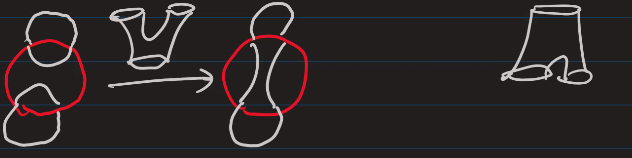
\includegraphics[width=0.8\linewidth]{seb3.png}
    \caption{Saddle cobordism}%
    \label{fig:seb2}
\end{figure}

To obtain $d^2 = 0$, we need that all square faces in the diagram anti-commute. The problem is that in the diagram, the two cobordisms are actually the same (we can reorder the saddles), so now we need to add signs to the edges such that each square face has an odd numbder of minus signs. In the example of the Hopf link, we just add a minus sign to the $10 \to 11$ edge.

Now we may construct the $m$-th chain group ${ [[L]] }^m$ of $[[L]]$ to be
\[ \bigoplus_{\alpha \mid \sum \alpha_i = m} (\text{resolution over $\alpha$}). \]
The chain homotopy type of $[[L]]$ is a link invariant after passing to a quotient $\ms{Cob}^3/\ell$ of $\ms{Cob}^3$ by the following relations:

\begin{figure}[H]
    \centering
    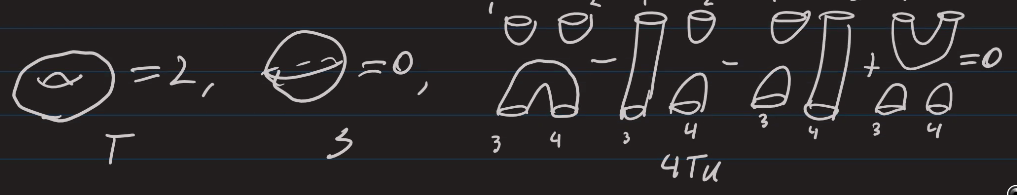
\includegraphics[width=0.8\linewidth]{seb5.png}
    \caption{Relations for $\ms{Cob}^3//\ell$}%
    \label{fig:seb3}
\end{figure}

Now we define the \textit{Bar-Natan category} $\ms{BN} \coloneqq \ms{Kom}(\ms{Mat}(\ms{Cob}^3/\ell))$. Of course, we now need to prove invariance under the Reidemeister moves. For the first Reidemeister move, we have the following diagram:

\begin{figure}[H]
    \centering
    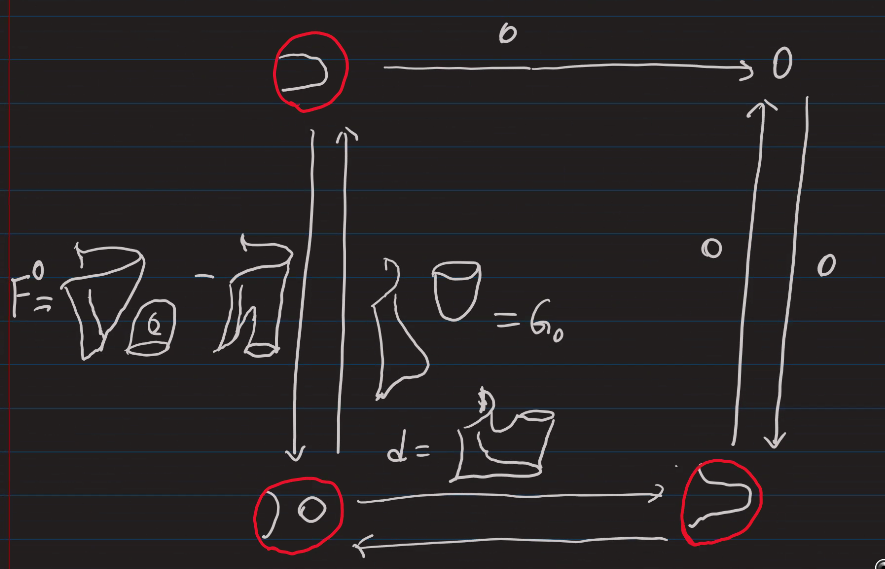
\includegraphics[width=0.6\linewidth]{seb6.png}
    \caption{Diagram for R1}%
    \label{fig:seb4}
\end{figure}

Then here hare the easy relations.

\begin{figure}[H]
    \centering
    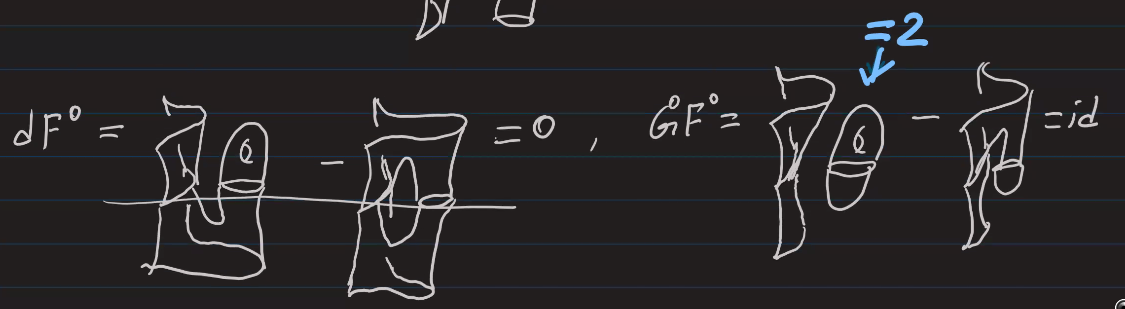
\includegraphics[width=0.8\linewidth]{seb7.png}
    \caption{Easy relations}%
    \label{fig:seb5}
\end{figure}

Finally, here we see that we have a homotopy:

\begin{figure}[H]
    \centering
    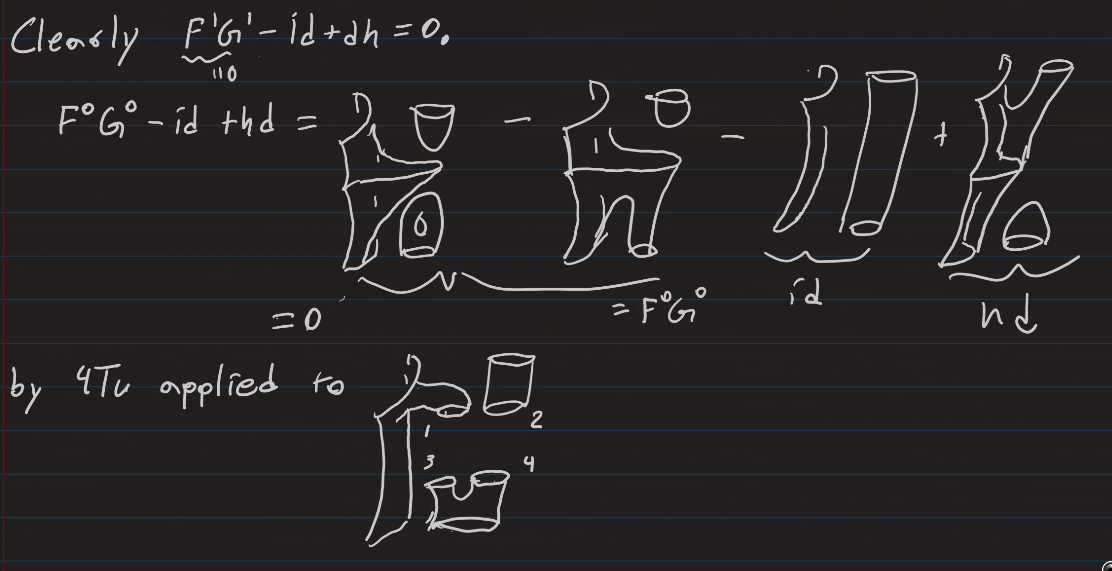
\includegraphics[width=0.8\linewidth]{seb8.png}
    \caption{The homotopy really is a homotopy}%
    \label{fig:seb6}
\end{figure}

The proofs of invariance under the other Reidemeister moves are similar, but significantly more complicated. But now any functor from $\ms{Cob}^3/\ell$ to any abelian category will give us a knot invariant. Note that such a functor does not have to be a $2$-dimensional TQFT.

\section{Khovanov Homology}%
\label{sec:khovanov_homology}

Returning to something more concrete, any cobordism in $\ms{Cob}^3/\ell$ can be decomposed into pairs of pants and caps and cups, so to specify a functor, we only need to specify what it does to four morphisms. Here, the cobordisms correspond to
\[ m \colon V \otimes V \to V \qquad \Delta \colon V \to V \otimes V \qquad \iota \colon V \to \Z \qquad \ep \colon V \to \Z, \]
where $V = \mc{F}(S^1)$ for $\mc{F}$ a TQFT. Then Khovanov homology is the functor where $V = \Z \qty{-1} \oplus \Z \qty{1}$, where $m$ is given by
\[ v_- \otimes v_- \mapsto 0 \qquad v_- \otimes v_+ \mapsto v_- \qquad v_+ \otimes v_+ \mapsto v_+ \qquad v_+ \otimes v_- \mapsto v_- ,\]
$\Delta$ is given by
\[ v_- \mapsto v_- \otimes v_- \qquad v_+ \mapsto v_+ \otimes v_- + v_- \otimes v_+, \]
$\iota$ is given by $1 \mapsto v_+$, and $\ep$ is given by $v_- \mapsto 1, v_+ \mapsto 0$. The grading on $V$ is called the \textit{Jones grading} because it records power of $q$ in the Jones polynomial.

Now we are finally able to define the Khovanov homology
\[ \mr{Kh}(L) \coloneqq H^*(\mc{F}([[L]]))[-n_-]\qty{n_+ - 2n_-} \]

\begin{thm}
    We have the formula
    \[ J(L) = \sum_{i,j} {(-1)}^i q^j \rk_{\Z} \mr{ Kh }^{i,j}(L). \]
\end{thm}

For the Hopf link, the chain complex is given by
\[ (V \otimes V)\qty{-4} \xrightarrow{m \oplus m} V \qty{-3} \oplus V\qty{-3} \xrightarrow{\Delta^1 - \Delta^2} (V \otimes V) \qty{-2}, \]
and thus we can compute the Khovanov homology.

\begin{thm}[Jacobsson, Bar-Natan]
    The map on $[[L]]$ associated to a cobordism in $\R^3 \times [0,1]$ is independent of its decomposition into elementary cobordisms up to a sign and cobordisms in the Bar-Natan category.
\end{thm}

\chapter{\'Alvaro (Sep 21): HOMFLY-PT homology}%
\label{cha:'alvaro_sep_21_homfly_pt_homology}

If we already know about Hecke algebras, then we could discover the HOMFLY-PT polynomial with the unknot being $1$ and the skein relation
\[ t \cdot \text{under} + t^{-1} \cdot \text{over} = z \cdot \text{unlinked}. \]
Here, if we set $t = q^{2N}$ and $z = q + q^{-1}$, we recover the $SL_2$ link polynomial and if we set $N = 1$, we recover the Jones polynomial.

The reason that we could have discovered the HOMFLY-PT polynomial is using the representation theory of the braid group, which is generated by $s_1, \ldots, s_{n-1}$ with relations $s_i s_{i+1} s_i = s_{i+1} s_i s_{i+1}$ and $s_i s_j = s_j s_i$ if $\abs{i-j} \geq 2$.

First, note that every link is the closure of a braid. Then two braids give rise to isotopic links if they are related by Markov moves. Now we consider
\[ \Z[q^{\pm}] \mr{Br}_n \twoheadrightarrow H(S_n) = \Z[q^{\pm}] \cdot \qty{\delta_w \mid w \in S_n} / \delta_s^2 = \delta_s (q-1) + q. \]
Now we can define a trace map
\[ \Tr \colon \bigcup_{n \geq 1} H(S_n) \to \Z[q^{\pm}, z^{\pm}] \]
with the condition that $\Tr(x s_n y) = z \Tr(xy)$ and $\Tr(1) = 1$. In particular, these imply that $\Tr(xy) = \Tr(yx)$, and this is called the \textit{Oceanu trace}. If we normalize the $s_i$, then $\Tr(x s_i) = \Tr(x s_i^{-1})$. Then under the correct normalization, we obtain the HOMFLY-PT polynomial.

\section{Triply graded homology}%
\label{sec:triply_graded_homology}

This was discovered by Khovanov-Rozansky in 2004 using matrix factorizations and Khovanov in 2005 using Soergel bimodules. Then work of various subsets of Elias, Hogancamp, and Mellit computed HHH for torus $(m,n)$-links.

Consider the symmetric group $S_m = \ev{s_1, \ldots, s_{m-1}}$. Then consider $R = \Q[x_1, \ldots, x_m]$, where the $x_i$ have degree $2$. Then we have a natural action of $S_m$ on $R$, and $R^{S_i}$ are the invariants. Then we will define $B_{s_i} = R \otimes_{R^s} R(1)$ as an $R$-bimodule, and for $\ul{w} = s_{i_1} \cdots s_{i_n}$, we will define the \textit{Bott-Samuelson bimodule} $BS(\ul{w}) = B_{s_{i_1}} \otimes \cdots \otimes B_{s_{i_n}}$. Next, if we consider the Bott-Samuelson bimodules and add in all tensor products and direct sums, we obtain the Hecke category $\ms{SBim}$, which categorifies the Hecke algebra.

In our running example, we will take $S_2 = \qty{1, s}$ and $R = \Q[x_1, x_2]$. Here, we will take $R^s = \Q[x_1+x_2, (x_1-x_2)^2]$, and we will write $r = x_1+x_2, t = x_1-x_2$. Therefore, we have
\[ BS(s^2) = B_s \otimes_R B_s = R \otimes_{R^s} R \otimes_R R \otimes_{R^s} R(2) = R \otimes_{R^s} R \otimes_{R^s} R(2). \]

\begin{thm}[Soergel's categorification theorem]
    Note that $H(S_n)$ has a KL-basis $\qty{b_w \mid w \in S_n}$. Then there is a bijection between indecomposables in $\ms{SBim}$ and the KL-basis taking the tensor product to multiplication.
\end{thm}

Now if we write $b_{s_i} = \delta_{s_i} + q$, we have $b_{s_i}^2 = q b_{s_i} + q^{-1} b_{s_i}$. On the other side, we have
\begin{align*}
    B_s^{\otimes 2} &= R \otimes_{R^2} \otimes R \otimes R(2) \\
    &= R \otimes (\Q[r,t^2] \oplus t \Q[r,t^2]) \otimes_{R^2} R(2) \\
    &= R \otimes_{R^s} R(2) \oplus R \otimes_{R^s} R \\
    &= B_s(1) \oplus B_s(-1).
\end{align*}

Now we will categorify the braid group and construct HHH. We have $b_s = \delta_s + q$ and thus $\delta_s = b_s - q$, so in the categorified version we will have $q_i \colon B_{s_i} \to R$. Then we consider the complex
\[ F_{s_i} = 0 \to \ul{B_{s_i}} \xrightarrow{q_i} R(1) \to 0 \to \cdots \]
and analogously
\[ F_{s_i}^{-1} = R(-1) \xrightarrow{d_i} \ul{B_{s_i}} \to 0 \to \cdots \]

\begin{thm}[Rouquier]
    The assignment $\ul{w} \to F^{\bullet}(\ul{w}) = F_{s_1^{\pm}} \otimes \cdots \otimes F_{s_{i_n}^{\pm}}$ is a well-defined homomorphism $\mr{Br}_n \to K^{b}(\ms{SBim})$.
\end{thm}

Now we apply the Hochschild homology $HH_n$ to $F^{\bullet}(w)$, and we obtain the complex
\[ HH_n(F^{-1}(w)) \to HH_n(F^0(w)) \to HH_n(F^1(w)), \]
and taking the homology, we obtain the HHH homology. The grading is given by the homological grading $HH_i(F^j(\ul{w}))$ that modifies $j$, the Hochschild grading, and the internal grading as $R$-graded bimodules.

\section{Hochschild homology}%
\label{sec:hochschild_homology}

Next we observe that Hochschild homology is easier for polynomial rings. Recall that if $R$ is a $k$-algebra, then if we write $R^{env} = R \otimes_k R^{op}$, we have
\[ HH_n(-) = \Tor_n^{R^{env}}(R,-). \]
Instead of the bar complex, we will consider the Koszul complex
\[ K^{\bullet} \bigwedge^n V \otimes R^{env} \to \cdots \to V \otimes R^{env} \to R^{env} \to R \to 0, \]
which is a free resolution of $R$, where $V = \Q^m$. Then this complex computes the Hochschild homology. For example, if $R = \Q[x] = M$ where $\deg x = 2$, we have
\[ K^{\bullet} = R^{env}(-2) \xrightarrow{(x \otimes 1 - 1 \otimes x)} R^{env} \] and $R(-2) \xrightarrow{0} R$, and thus
\[ HH_*(R) = \begin{cases}
    \Q[x] & * = 0 \\ 
    \Q[x](-2) & * = 1.
\end{cases}
\]

for another example, when $R = \Q[x,y]$ and $M$ is a graded $R$-bimodule, and $\deg x = \deg y \ 2$, we have
\[ K^{\bullet} = R^{env}(-4) \to R^{env}(-2) \oplus R^{env}(-2) \to R^{env} \]
where the maps are given by $(x \otimes 1 - 1 \otimes x, 1 \otimes y - y \otimes 1)$ and $(y \otimes 1 - 1 \otimes y, x \otimes 1 - 1 \otimes x)$, and the Koszul resolution of $M$ is similar.

\section{Example of triply graded homology}%
\label{sec:example_of_triply_graded_homology}

Now the unknot is the closure of $1 \in \mr{Br}_1$, and so we want to compute its homology $HHH_{***}$. We know that
\[ F^{\bullet}(1) = 0 \to \ul{R} \to 0, \]
and therefore
\[ HH_*(R) = \begin{cases}
    \Q[x] & * = 0 \\ 
    \Q[x](-2) & * = 1.
\end{cases}
\]
The Euler characteristic is
\[ (1 + q^2 + q^4 + \cdots) + a (q^2 + q^4 + \cdots) = \frac{1+aq^2}{1-q^2}, \]
and this recovers the unknot.

Now if we take the closure of $s \in \mr{Br}_2$, which is still the unknot, we have
\[ F^{\bullet}(S) = \ul{B_s} \to R(1) ,\]
where $R = \Q[x_1, x_2]$. But now we need to compute the Hochschild homology
\[ HH_*(B_s) \to HH_*(R(1)) \]
in all degrees. For $R(1)$, the Koszul resolution is
\[ R(-3) \xrightarrow{0} { R(-1) }^{\oplus 2} \xrightarrow{0} R(-1) \]
and for $B_s$ it is
\[ B_s(-4) \xrightarrow{(f,f)} B_s(-2) \oplus B_s(-2) \xrightarrow{(-f,f)} B_s, \]
where $R^s = \Q[s,t^2]$ and $f(m) = \frac{1}{2} tm - \frac{1}{2} mt$. Now we have $\ker(f) = \ev{mt+tm}, \Im(f) = mt-tm$. Now we compute $HH_0(B_s) = B_s/\Im f$, $HH_*(B_s) = R(-1) \oplus \ker(f)(-2)$, and $HH_2(B_s) = \ker(f)(-4)$. Then the three maps are the identity in degree $0$, $(\mr{id}, i)$ in degree $1$, and $i$ in degree $2$, where $i$ is the counit. Finally we obtain the following table for the HHH:
\begin{table}[H]
    \centering
    \caption{HHH homology}
    \label{tab:label}
    \begin{tabular}{ccc}
    \toprule
    Hochschild degree & $HHH_{0**}(s_1)$ & $HHH_{1**}(s_1)$ \\
    \midrule
        $0$ & $0$ & $0$ \\
        $1$ & $0$ & $\Q[r](-1)$ \\
        $2$ & $0$ & $\Q[r](-3)$
    \end{tabular}
\end{table}

This is isomorphic to $HHH(1)$ in the previous example after a shift.

Finally consider the Hopf link, which is the closure of $s^2$. Here $F^{\bullet}(s^2)$ is given by
\begin{equation*}
\begin{tikzcd}
    B_s^{\otimes 2} \ar{r} \ar{d} & B_s(-1) \ar{d} \\
    B_s(1) \ar{r} & R(2).
\end{tikzcd}
\end{equation*}
This complex is homotopic to $B_s(-1) \to B_s(1) \to R(2)$.

\section{Connections to geometry}%
\label{sec:connections_to_geometry}

Define the matrix $B_i(z)$ to have the matrix $\begin{psmallmatrix}
    0 & 1 \\ 1 & z
\end{psmallmatrix}$ in the $i$-th position. Then we have the identity
\[ B_i(z_1) B_{i+1}(z_2) B_i(z_3) = B_{i+1}(z_3) B_i(z_2 - z_1 z_3) B_{i+1}(z_1). \]
For a positive braid $\beta = s_{i_1} \cdots s_{i_n}$, we assign the matrix $B_{\beta}(z_1, \ldots, z_n) = B_{i_1}(z_1) \cdots B_{i_n}(z_n)$, and finally we consider the variety 
\[ X(\beta) = \qty{(z_1, \ldots, z_n) \in \C^n \mid B_{\beta}(z_1, \ldots, z_n) \text{ is upper triangular}}. \]
For example, if $\beta$ is the trefoil knot, then $X(\beta) = \qty{1 + z_1 z_2 = 0}$. There is a torus action on this variety, where if we have $n$ strands there is an action of ${(\C^{\times})}^{n-1}$. In this example, we have $(z_1, z_2, z_3) \mapsto (z_1 \cdot t, z_2 \cdot t^{-1}, z_3)$.

\begin{thm}[Trinh, 2021]
    We have $H_{*,BM}^T(X(\beta))$ has a nontrivial weight filtration whose associated graded module is isomorphic to $HHH_{0**}(\beta)$.
\end{thm}

For the trefoil knot, we obtain a grading on $H_*(S^1)$.

Finally, relating this to Hilbert schemes we have the Oblomkov-Shende conjecture, where if $C$ is an integral plane curve and $p$ is a singularity, then
\[ \mr{HOMFLY}(\mr{link}(p)) = {\qty(\frac{a}{q})}^{\mu - 1} \sum_{\ell,m} q^{2\ell} {(-a^2)}^m \chi(C_p^{[\ell,\ell+m]}). \]
Next, there is the Oblomkov-Rasmussen-Shende conjecture, which says that replacing $\chi$ with $H^*$, we obtain HHH. Then there is Oblomkov-Rozansky homology, and finally a conjecture of Gorsky-Negut-Rasmussen, which says that if $X = F \mr{Hilb}_n^{dg}(\A^2)$ is a dg version of the flag Hilbert scheme, then there is a commutative diagram of monoidal functors
\begin{equation*}
\begin{tikzcd}
    K^b(\ms{SBim}_n) \ar{r}{L_*} \ar{d}{HHH} & D^b(\ms{Coh}_{\C^{\times} \times \C^{\times}}(X)) \\
    \ms{Vect}_{\Q}^{\Z^{\oplus 3}},
\end{tikzcd}
\end{equation*}
where $\ms{Vect}_{\Q}^{\Z^{\oplus 3}}$ is the category of $\Z^{\oplus 3}$-graded $\Q$-vector spaces.

\chapter{Avi (Sep 28): Hilbert Schemes}%
\label{cha:avi_sep_28_hilbert_schemes}

\section{Definitions}%
\label{sec:definitions}

Let $X$ be a projective variety over a field $k = \C$. For example, if $X = \P^n$, we in algebraic geometry are interested in projective varieties, which are closed subschemes of $X$. We are interested in classifying closed subschemes of $X$, and to do this we will construct a functor $\mr{Hilb}(X)$ given by
\[ \Hilb(X)(T) = \qty{ Z \subset T \times X \mid Z \to T \text{ flat}}. \]
We are interested in the representability of this functor, and unfortunately this functor is not representable in any reasonable way.

For example, consider $X = \P^1$. If we consider subschemes with finite support, we obtain the space
\[ \bigsqcup_n \mr{Sym}^n \P^1 = \bigsqcup_n \P^n. \]
This has infinitely many connected components and is infinite-dimensional in general. This tells us that we want to stratify our functor into pieces.

Now consider $Z \subset X = \P^n$. Then define graded coordinate ring $R = \bigoplus_i R_i$ of $Z$ and the function $i \mapsto \dim_R R_i$. For $i \gg 0$, this function equals some polynomial in $i$. More generally, let $\mc{F}$ be a quasicoherent sheaf on $X$. Then we can consider the function
\[ i \mapsto h^0(X, \mc{F}(i)), \]
and in particular, for $i \gg 0$, this function equals the Euler characteristic $\chi(\mc{F}(i))$ because for $i$ sufficiently large, all twists have vanishing higher cohomology. Finally, $\chi(\mc{F}(i))$ is a polynomial, which we will call the \textit{Hilbert polynomial} $P_{\mc{F}}(i)$.

For a subscheme $Z \subset X$ with ideal sheaf $\mc{I}_Z \subseteq \mc{O}_X$, we will define $P_Z = P_{\mc{I}_Z}$. Returning to $X = \P^1$, then if $Z$ is a scheme which is $n$ points, then $\dim H^0(X, \mc{I}_Z) = n$. For the subscheme $X$, we have $h^0(X, \mc{O}_X(i)) = i+1$. We are now able to define the functor
\[ \Hilb^f(X)(T) \coloneqq \qty{Z \subseteq T \times X \mid Z \to T \text{ flat}, P_{Z_t} = f}. \]
In particular, we have a decomposition
\[ \Hilb(X) = \bigsqcup_f \Hilb^f(X). \]
In our case, we will focus on $0$-dimensional subschemes, and we will denote both the functor and the scheme that represents it as $X^{[n]} = \Hilb^n(X)$.

\begin{exm}
    Suppose $n = 0$. All subschemes of $T \times X$ with $P_{Z_t} = 0$ must have empty fibers over $T$ and thus must be empty themselves.

    If $n = 1$, then all ideals of colength $1$ are maximal ideals, which are the same as closed points of $X$, so $X^{[1]} = X$.

    When $n = 2$, we are looking for ideals $\mc{I}$ such that $\mc{O}_X / \mc{I}$ has length $2$. Thus either this subscheme is supported at two distinct points or a single point. If the support of the subscheme is two distinct points $x_1 \neq x_2$, then at each $x_i$, the ring $\mc{O}_X/\mc{I}$ must have length $1$. Thus we have a locus $(X \times X \setminus \Delta) / S_2$. In the second case, where $\mc{O}_X / \mc{I}$ is supported at a single point $x$, then we have a sequence of inclusions
    \[ \mf{m}_x^2 \subseteq I \subset \mc{m}_X \subset \mc{O}_X. \]
    Thus we are looking for morphisms $\varphi \colon \mf{m}_x / \mf{m}_x^2 \to k$ up to a scalar, so above the point $x$ we have $\P T_{X,x}$, and therefore we have
    \[ X^{[2]} = (X \times X \setminus \Delta) / S_2 \sqcup \P T_X. \]
\end{exm}

More generally, we have a morphism $\pi \colon X^{[n]} \to \mr{Sym}^n X$ sending a subscheme $Z$ to its support $\abs{Z}$, called the \textit{Hilbert-Chow morphism}. If $\lambda = (\lambda_1, \ldots, \lambda_r)$ is a partition of $n$, we have a stratum $\Sym^{\lambda} X$ with fixed multiplicities given by $\lambda$. Thus we have
\[ \Sym^n X = \bigsqcup_{\lambda} \Sym^{\lambda} X, \]
which induces a stratification of $X^{[n]}$ into pieces $X_{\lambda}^{[n]}$.

For example, when $\lambda = (n)$, we have the Hilbert-Chow morphism
\[ X_{(n)}^{[n]} \xrightarrow{\pi} \Sym^{(n)} X = X, \]
and so the fibers are schemes $X_p^{[n]}$ parameterizing length $n$ subschemes of $X$ supported at $p$.

\begin{exm}
    When $X$ is a smooth curve, $\pi$ is actually an isomorphism. This is because all local rings $\mc{O}_{X,p}$ are discrete valuation rings, and in particular they have a unique idea of length $n$. Therefore all fibers of $\pi$ must be points.
\end{exm}

When $X$ is a smooth surface, then $X^{[n]}$ is always smooth, but in fact Hilbert schemes of points are highly singular for $n > 2$ in higher dimension.

\section{Hilbert schemes of smooth surfaces}%
\label{sec:hilbert_schemes_of_smooth_surfaces}

Now suppose that $X$ is a smooth surface. Suppose that $Z \subseteq X$ is supported at a point $p$ with length $n$. In particular, we have a chain of inclusions
\[ \mf{m}_x^n \subseteq I \subseteq \mf{m}_x^{n-1} \subset \mc{O}_{X,x}, \]
and thus this data is equivalent to $I / \mf{m}_x^n \subset \mc{O}_{X,x} / \mf{m}_x^{n-1}$. Up to completion, all of this data is independent of both $X$ and $x$, and in fact
\[ \wh{\mc{O}}_{X,x} = k[[T_1, T_2]]. \]
Therefore, $X_x^{[n]}$ is independent of $X,x$, so we may consider $X = \A^2, x = 0$. We will see that ${(\A^2)}_0^{[n]}$ has dimension $n-1$. In general, we have
\begin{align*} 
    \dim X_{(\lambda_1, \ldots, \lambda_r)}^{[n]} &= \dim X_{(\lambda_1)}^{[\lambda_1]} + \cdots + \dim X_{(\lambda_r)}^{[\lambda_r]} \\
    &= \dim X + \dim X_p^{[\lambda_1]} + \cdots \\
    &= (\lambda_1 + 1) + \cdots + (\lambda_r + 1) \\
    &= n + r.
\end{align*}
In particular, $\dim X^{[n]} = 2n$.

Now we will compute the tangent space of $X^{[n]}$. If a subscheme $Z$ is given by an ideal $\mc{I}$, we first show that the tangent space to $X^{[n]}$ at $\mc{I}$ is given by $\Hom(\mc{I}, \mc{O}_X/\mc{I})$, and then we can use Hirzebruch-Riemann-Roch. Alternatively, consider the action of $G_m \times G_m$ on $\A^2$. This lifts to an action on ${(\A^2)}^{[n]}$, and the fixed points are given by monomial ideals. Each monomial ideal corresponds to a Young diagram (just consider all monomials not in the ideal), and of course these are in bijection with partitions of $n$. If we do some allegedly very elegant combinatorics, we obtain the desired result.

We will now connect Hilbert schemes of surfaces to representation theory. We have the formula of G\"ottsche, which states that
\[ \sum_{n = 0}^{\infty} \sum_{i=0}^{4n} b_i(X^{[n]}) t^i q^n = \prod_{m=1}^{\infty} \prod_{j=0}^4 {(1- {(-1)}^j t^{2m+j-2} q^m)}^{-{(-1)}^i b_j(X)} \]
and another formula which states that
\[ \sum_{n=0}^{\infty} \chi(X^{[n]}) q^n = \prod_{j=0}^4 {\qty(\prod_{m \geq 1} (1-q^m))}^{-{(-1)}^i b_j(X)}. \]
In particular, doing some generatingfunctionology gives us the Betti numbers.

These formulas are similar to those coming from representations of the Heisenberg algebra. In fact, the total cohomology of the Hilbert scheme is a representation of the Heisenberg algebra. We consider the incidence schemes
\[ X^{[n, \ell]} \subset X^{[n]} \times X^{[n+\ell]} \]
which classifies subschemes $Z_1 \subset Z_2$ which differ at a single point $x$.

\section{Plane curve singularities}%
\label{sec:plane_curve_singularities}

There exists a similar formula to those of G\"ottsche for smooth curves due to Macdonald, which says that
\[ \sum_{n=0}^{\infty} \chi(C^{[n]}) q^n = {(1-q)}^{-\chi(C)}. \]
We would like to say something about the LHS, which we will call $W(C)$, in general when $C$ is not smooth. Write $C = C_{\mr{sm}} \cup \qty{p_i}$, where the $p_i$ are the singularities of $C$. Then we have
\[ W(C) = W(C_{\mr{sm}}) \prod_{n=0}^{\infty} \chi(C_p^{[n]}) q^n \]
by the cut-and-paste relation for the Euler characteristic. To make sense of what happens at the singular points, we will consider knot theory.

Near $p \subset C \subset \C^2$, we will consider $C \cap S^3$, which has real dimension $1$ and is therefore a link $L_p$. We would hope that some knot invariant of $L_p$ will recover the data of the fomula above, and according to the Oblomkov-Shende conjecture, this is true. The conjecture says that
\[ \sum_{n=0}^{\infty} \chi(C_p^{[n]}) q^{2n} = \lim_{t \to 0} {\qty(\frac{q}{t})}^{\mu} P(L_p), \]
where $P$ is the HOMFLY polynomial. To recover the entire Homfly polynomial, we have an upgraded version of the conjecture, which says that
\[ P(L_p) = {\qty(\frac{t}{q})}^{\mu} (1-q^2) \sum_{m,n} \chi(C_{p,m}^{[n]}) {(1-t^2)}^{m-1} q^{2n}, \]
where $C_{p,m}^{[n]}$ parameterizes colength $n$ ideals $\mc{I}$ generated by $m$ elements. This conjecture is known for torus knots and in the special case when $t = 1$, among others.



\end{document}
